% !TEX program = lualatex
\documentclass[11pt,a4paper]{article}

%% ----------------------------------------------------------------
%%  Packages
%% ----------------------------------------------------------------
\usepackage[margin=2.4cm]{geometry}
\usepackage{amsmath,amssymb,amsthm}
\usepackage{mathtools}
\usepackage{bm}
\usepackage{algorithm}
\usepackage{algpseudocode}
\usepackage{booktabs}
\usepackage{multirow}
\usepackage{array}
\usepackage{colortbl}
\usepackage{xcolor}
\usepackage{graphicx}
\usepackage{tikz}
\usepackage{tikz-cd}
\usepackage{pgfplots}
\pgfplotsset{compat=1.18}
\usetikzlibrary{arrows.meta,calc,positioning,shapes.geometric,
                 decorations.pathmorphing,fit,backgrounds,
                 patterns,shadows,matrix}
\usepackage[colorlinks=true,linkcolor=blue!60!black,
            citecolor=green!50!black,urlcolor=blue!70!black]{hyperref}
\usepackage{caption}
\usepackage{subcaption}
\usepackage{float}
\usepackage{enumitem}
\usepackage{microtype}

%% ----------------------------------------------------------------
%%  Custom colours
%% ----------------------------------------------------------------
\definecolor{motoblue}{HTML}{1565C0}
\definecolor{motoorange}{HTML}{E65100}
\definecolor{motogreen}{HTML}{2E7D32}
\definecolor{motored}{HTML}{C62828}
\definecolor{motogray}{HTML}{546E7A}
\definecolor{valhallagold}{HTML}{F9A825}
\definecolor{passbg}{HTML}{E8F5E9}
\definecolor{failbg}{HTML}{FFEBEE}

%% ----------------------------------------------------------------
%%  Math short-hands
%% ----------------------------------------------------------------
\newcommand{\WW}{\mathcal{W}}
\newcommand{\GG}{\mathcal{G}}
\newcommand{\EE}{\mathcal{E}}
\newcommand{\VV}{\mathcal{V}}
\newcommand{\CC}{\mathrm{CC}}
\DeclareMathOperator*{\argmin}{arg\,min}

\theoremstyle{definition}
\newtheorem{definition}{Tan{\i}m}[section]
\newtheorem{proposition}{\"Onerme}[section]

%% ----------------------------------------------------------------
\title{\textbf{MOTOMAP: Motosiklet Odakl{\i} Ak{\i}ll{\i} Rota
       Optimizasyon Motoru}\\[6pt]
       \large Algoritma Do\u{g}rulama, Sistem Mimarisi ve
              Benchmark Raporu}
\author{Ali \"Ozuysal \and Muhammet Ya\u{g}c{\i}o\u{g}lu}
\date{5 Mart 2026}

\begin{document}
\maketitle

%% ================================================================
%%  ABSTRACT
%% ================================================================
\begin{abstract}
Mevcut navigasyon sistemleri t\"um ara\c{c} tiplerini otomobil merkezli
tek bir trafik modeliyle de\u{g}erlendirmekte ve motosikletlerin fiziksel
avantajlar{\i}n{\i} (\"orne\u{g}in \c{c}ok \c{s}eritli yollarda \c{s}erit
aras{\i}nda ilerleme) ve yasal k{\i}s{\i}tlamalar{\i}n{\i}
(d\"u\c{s}\"uk CC motorlara otoyol yasa\u{g}{\i}) g\"oz ard{\i}
etmektedir. MOTOMAP, motosiklet dinami\u{g}ini matematiksel olarak
modelleyen \"ozel bir rota optimizasyon motorudur. Bu rapor; \c{s}erit
filtreleme (lane filtering), motor hacmi (CC) bazl{\i} e\u{g}im cezas{\i},
otonom hata kurtarma (resilience) ve g\"uvenlik odakl{\i} viraj analizi
\"ozelliklerinin mimarisini detayland{\i}rmaktad{\i}r.
End\"ustri standartlar{\i} (Google~Maps ve Valhalla) ile yap{\i}lan
\emph{benchmark} testleri, MOTOMAP'in ortalama $\mathord{\sim}\!5\%$
s\"ure avantaj{\i} sa\u{g}lad{\i}\u{g}{\i}n{\i} ve motosiklete \"ozg\"u
k{\i}s{\i}tlamalarda $100\%$ do\u{g}rulukla \c{c}al{\i}\c{s}t{\i}\u{g}{\i}n{\i}
kan{\i}tlam{\i}\c{s}t{\i}r.
\end{abstract}

\tableofcontents
\newpage

%% ================================================================
%%  1.  INTRODUCTION
%% ================================================================
\section{Giri\c{s} ve Proje Vizyonu}\label{sec:intro}

Navigasyon end\"ustrisinde standart kabul edilen uygulamalar
(Google~Maps, Yandex, Apple~Maps), trafikteki t\"um ara\c{c}lar{\i}
homojen bir h{\i}z modeliyle varsayar. Bu varsay{\i}m, bir otomobilin
veya bir kamyonun bo\c{s} bir otoyoldaki davran{\i}\c{s}{\i}n{\i}
yakalamakta yeterliyken, bir motosikletin s{\i}k{\i}\c{s}{\i}k trafikte
\c{s}eritler aras{\i}nda ilerleyerek elde etti\u{g}i s\"ure avantaj{\i}n{\i}
tamamen g\"ozard{\i} eder.

MOTOMAP, bu asimetriyi ``\c{S}erit Filtreleme'' (lane filtering) h{\i}z
modeliyle yakalayan, motor hacmine (CC) g\"ore yasal
k{\i}s{\i}tlamalar{\i} otomatik uygulayan ve rotadaki viraj
geometrisini motos\"ur\"uc\"u perspektifinden analiz eden bir
\emph{karar destek sistemi} olarak tasarlanm{\i}\c{s}t{\i}r.

%% ================================================================
%%  2.  MATHEMATICAL MODELS
%% ================================================================
\section{Matematiksel Modeller ve Maliyet Fonksiyonu}\label{sec:math}

\subsection{Bile\c{s}ik Maliyet A\u{g}{\i}rl{\i}kland{\i}rmas{\i}}

Sistem, rota optimizasyonunda standart Dijkstra algoritmas{\i}n{\i}
motosiklete \"ozg\"u bir bile\c{s}ik maliyet a\u{g}{\i}rl{\i}\u{g}{\i}
$\WW(e)$ ile geni\c{s}letir.

\begin{definition}[Kenar maliyet fonksiyonu]
$\GG=(\VV,\EE)$ otonom y\"onl\"u bir \c{c}izge olsun. Her $e=(u,v)\in\EE$
kenar{\i} i\c{c}in bileşik maliyet:
\begin{equation}\label{eq:cost}
  \WW(e)
  \;=\;
  T_{\mathrm{moto}}(e)
  \;\cdot\;
  C_{\mathrm{otoban}}(e)
  \;\cdot\;
  C_{\mathrm{e\u{g}im}}(e)
  \;\cdot\;
  C_{\mathrm{mod}}(e)
\end{equation}
olarak tan{\i}mlan{\i}r; burada
$T_{\mathrm{moto}}$ motosiklet seyir s\"uresi,
$C_{\mathrm{otoban}}$ otoban k{\i}s{\i}tlama \c{c}arpan{\i},
$C_{\mathrm{e\u{g}im}}$ e\u{g}im ceza \c{c}arpan{\i} ve
$C_{\mathrm{mod}}$ s\"ur\"u\c{s} modu (standart/viraj/g\"uvenli)
\c{c}arpan{\i}d{\i}r.
\end{definition}

\subsection{Motosiklet Seyir S\"uresi: \c{S}erit Filtreleme Modeli}

Trafik ak{\i}\c{s} h{\i}z{\i} $V_{\mathrm{araba}}$ \c{s}ehir
i\c{c}inde belirli bir e\c{s}ik de\u{g}erin alt{\i}na
d\"u\c{s}t\"u\u{g}\"unde ($V_{\mathrm{araba}} < 10\;\mathrm{km/h}$),
motosiklet gidi\c{s} y\"on\"undeki \c{s}erit say{\i}s{\i}na
($n_{\text{şerit}}$) ba\u{g}l{\i} olarak manevra avantaj{\i} elde eder:
\begin{equation}\label{eq:filter}
  V_{\mathrm{moto}}
  \;=\;
  \begin{cases}
    V_{\mathrm{araba}} + 5
      & n_{\text{şerit}} = 1,\\[4pt]
    \max\!\big(V_{\mathrm{araba}} + 15,\; 25\big)
      & n_{\text{şerit}} = 2,\\[4pt]
    \max\!\big(V_{\mathrm{araba}} + 20,\; 35\big)
      & n_{\text{şerit}} \ge 3.
  \end{cases}
\end{equation}
Gidi\c{s} y\"on\"u \c{s}erit say{\i}s{\i}; tek y\"onl\"u yolda
toplam \c{s}erit say{\i}s{\i}na, \c{c}ift y\"onl\"u yolda ise
$\max(1,\lfloor n_{\text{toplam}}/2\rfloor)$ de\u{g}erine e\c{s}ittir.

\subsection{CC Bazl{\i} E\u{g}im Ceza Fonksiyonu}

Motor hacmi ($\CC$) ile e\u{g}im ($|\alpha|$) aras{\i}ndaki ceza
ili\c{s}kisi par\c{c}al{\i} bir fonksiyon olarak modellenmi\c{s}tir.
50\,cc ve alt{\i} motorlar{\i}n otoyol eri\c{s}imi
$C_{\mathrm{otoban}}=\infty$ ile engellenirken, e\u{g}im cezas{\i}
\c{s}\"oyle tan{\i}mlan{\i}r:

\begin{equation}\label{eq:cc_grade}
  C_{\mathrm{e\u{g}im}}(|\alpha|,\,\CC)
  \;=\;
  \begin{cases}
    6.0 & \CC\le 50,\;|\alpha|>0.12\\
    3.0 & \CC\le 50,\;0.08<|\alpha|\le 0.12\\
    2.0 & \CC\le 50,\;0.06<|\alpha|\le 0.08\\
    1.35& \CC\le 50,\;0.04<|\alpha|\le 0.06\\[6pt]
    2.0 & 50<\CC<250,\;|\alpha|>0.12\\
    1.5 & 50<\CC<250,\;0.09<|\alpha|\le 0.12\\
    1.2 & 50<\CC<250,\;0.06<|\alpha|\le 0.09\\[6pt]
    1.35& \CC\ge 250,\;|\alpha|>0.14\\
    1.15& \CC\ge 250,\;0.10<|\alpha|\le 0.14\\
    1.0 & \text{di\u{g}er}
  \end{cases}
\end{equation}

\noindent Bu fonksiyonun s\"ureklili\u{g}i \c{S}ekil~\ref{fig:grade-penalty}
ile g\"orsel\-le\c{s}tirilmi\c{s}tir.

\begin{figure}[H]
\centering
\begin{tikzpicture}
\begin{axis}[
    width=0.78\textwidth, height=6cm,
    xlabel={Mutlak e\u{g}im $|\alpha|$},
    ylabel={$C_{\mathrm{e\u{g}im}}$},
    xmin=0, xmax=0.18,
    ymin=0.8, ymax=6.5,
    grid=major,
    legend pos=north west,
    legend style={font=\small, fill=white, fill opacity=0.85},
]
% CC <= 50
\addplot[motored, very thick, const plot]
  coordinates {(0,1)(0.04,1.35)(0.06,2.0)(0.08,3.0)(0.12,6.0)(0.18,6.0)};
\addlegendentry{$\CC\le 50$}
% 50 < CC < 250
\addplot[motoblue, very thick, dashed, const plot]
  coordinates {(0,1)(0.06,1.2)(0.09,1.5)(0.12,2.0)(0.18,2.0)};
\addlegendentry{$50<\CC<250$}
% CC >= 250
\addplot[motogreen, very thick, dotted, const plot]
  coordinates {(0,1)(0.10,1.15)(0.14,1.35)(0.18,1.35)};
\addlegendentry{$\CC\ge 250$}
\end{axis}
\end{tikzpicture}
\caption{CC s{\i}n{\i}f{\i}na g\"ore e\u{g}im ceza \c{c}arpan{\i}n{\i}n
         $|\alpha|$ ile de\u{g}i\c{s}imi.}
\label{fig:grade-penalty}
\end{figure}

\subsection{Viraj Analizi: Vekt\"orel A\c{c}{\i} Hesaplamas{\i}}

Her $e \in \EE$ kenar{\i}n{\i}n LineString geometrisi,
$\Delta s = 10$\,m ad{\i}mlarla yeniden \"orneklenir. Ard{\i}\c{s}{\i}k
noktalar aras{\i}ndaki ard{\i}\c{s}{\i}k y\"on vekt\"orleri
$\mathbf{v}_i = \mathbf{p}_{i+1}-\mathbf{p}_i$ tan{\i}mlan{\i}r ve
sapma a\c{c}{\i}s{\i}:
\begin{equation}\label{eq:angle}
  \theta_i
  \;=\;
  \arccos\!\left(
    \frac{\mathbf{v}_i \cdot \mathbf{v}_{i+1}}
         {\|\mathbf{v}_i\|\;\|\mathbf{v}_{i+1}\|}
  \right)
\end{equation}
hesaplan{\i}r. A\c{c}{\i}lar \"u\c{c} s{\i}n{\i}fa a\c{c}{\i}l{\i}r:

\begin{table}[H]
\centering
\caption{Viraj a\c{c}{\i}s{\i} s{\i}n{\i}fland{\i}rmas{\i} ve anlam{\i}.}
\label{tab:angle-class}
\renewcommand{\arraystretch}{1.3}
\begin{tabular}{lccl}
\toprule
\textbf{S{\i}n{\i}f} & \textbf{Alt s{\i}n{\i}r} & \textbf{\"Ust s{\i}n{\i}r}
  & \textbf{Anlam} \\
\midrule
\rowcolor{passbg}
\emph{Fun} (keyifli) & $15°$ & $45°$ & Ak{\i}c{\i}, e\u{g}lenceli viraj \\
\emph{Tehlikeli}      & $60°$ & --- & Keskin d\"on\"u\c{s} \\
\rowcolor{failbg}
\emph{Hairpin}         & $60°$ & --- & $\Delta s_{\text{ard{\i}\c{s}{\i}k}} \le 20$\,m \\
\bottomrule
\end{tabular}
\end{table}

\noindent Y\"uksek risk b\"olgesi, tehlikeli viraj ile dik ini\c{s}in
kesi\c{s}imi olarak tan{\i}mlan{\i}r:
\begin{equation}\label{eq:highrisk}
  \mathcal{R}(e)
  \;=\;
  \bigl[\,n_{\text{hairpin}}(e)>0\bigr]
  \;\wedge\;
  \bigl[\,\text{grade}(e) < -0.08\bigr].
\end{equation}

%% ================================================================
%%  3.  MODE-SPECIFIC COST MODELS
%% ================================================================
\section{S\"ur\"u\c{s} Modlar{\i} ve Maliyet Formalizasyonu}\label{sec:modes}

MOTOMAP \"u\c{c} s\"ur\"u\c{s} modu sunar; her mod, kenar
a\u{g}{\i}rl{\i}\u{g}{\i}n{\i} farkl{\i} bir ama\c{c} fonksiyonuyla
yeniden tan{\i}mlar.

\begin{definition}[Yo\u{g}unluk doyurma fonksiyonu]\label{def:sat}
$x\ge 0$ i\c{c}in doyurma (saturation) fonksiyonu:
\begin{equation}\label{eq:sat}
  \sigma(x) = \frac{x}{2+x},
  \qquad
  \sigma:\mathbb{R}_{\ge 0}\to [0,1).
\end{equation}
\end{definition}

\noindent Viraj yo\u{g}unluklar{\i}
$\rho_{\text{fun}}=n_{\text{fun}}/\ell_{\text{km}}$ ve
$\rho_{\text{teh}}=n_{\text{teh}}/\ell_{\text{km}}$ tan{\i}mlanarak,
modlara g\"ore maliyet \c{s}\"oyle verilir:

\smallskip\noindent\textbf{Standart mod.}
Salt seyir s\"uresi minimizasyonu; yol tipi bazl{\i}
ek cezayla:
\begin{equation}\label{eq:standart}
  \WW_{\text{std}}(e) = T_{\mathrm{moto}}(e)
    \cdot C_{\mathrm{e\u{g}im}}
    \cdot C_{\mathrm{otoban}}
    \cdot \bigl(1 + p_{\text{yol}}\bigr).
\end{equation}

\smallskip\noindent\textbf{Viraj keyfi modu.}
Ak{\i}c{\i} virajl{\i} yollar{\i} \"od\"ullendiren; tehlikeli
virajlar{\i} cezaland{\i}ran form\"ulasyon:
\begin{equation}\label{eq:viraj}
  \WW_{\text{viraj}}(e) =
    \frac{T_{\mathrm{moto}}(e)\cdot C_{\mathrm{e\u{g}im}}\cdot C_{\mathrm{otoban}}}
         {\underbrace{1 + 0.95\,\kappa + 0.70\,\sigma(\rho_{\text{fun}}) + b_{\text{yol}}}_\text{bonus}}
    \;\cdot\;
    \underbrace{\bigl(1 + 0.25\,\sigma(\rho_{\text{teh}}) + 0.45\,\mathcal{R}\bigr)}_\text{ceza}
\end{equation}
burada $\kappa = s/(1+s)$ normalize edilmi\c{s} kıvrımlılık
skoru ve $b_{\text{yol}}$ yol tipi bonusudur.

\smallskip\noindent\textbf{G\"uvenli mod.}
Riskli segmentleri izole eden savunmac{\i} routing:
\begin{equation}\label{eq:guvenli}
  \WW_{\text{g\"uv}}(e) =
    T_{\mathrm{moto}}(e)\cdot C_{\mathrm{e\u{g}im}}\cdot C_{\mathrm{otoban}}
    \;\cdot\;
    \bigl(1 + 0.55\,\sigma(\rho_{\text{teh}}) + 1.40\,\mathcal{R}
          + 5.00\,\delta_{\text{ini\c{s}}}
          + p_{\text{yol}}\bigr)
\end{equation}
ile $\delta_{\text{ini\c{s}}} = \max\bigl(0,\;|\min(0,\alpha)|-0.08\bigr)$.

\begin{figure}[H]
\centering
\begin{tikzcd}[column sep=3.2em, row sep=2.6em]
  T_{\mathrm{moto}}
    \arrow[r,"\times"]
    \arrow[d,"\text{temel s\"ure}"']
  & C_{\mathrm{e\u{g}im}} \cdot C_{\mathrm{otoban}}
    \arrow[r,"\text{mod se\c{c}imi}"]
    \arrow[d,"\text{fiziksel k{\i}s{\i}tlama}"']
  & |[draw,rounded corners,fill=motoblue!10]| \WW_{\text{std}}
    \arrow[d, bend left=15, "\text{min}(T)"]\\
  \sigma(\rho_{\text{fun}})
    \arrow[r,"\text{bonus}"]
  & |[draw,rounded corners,fill=motogreen!10]|
    \WW_{\text{viraj}}
    \arrow[r, "\text{max(keyif)}"]
  & |[draw,rounded corners,fill=motored!10]|
    \WW_{\text{g\"uv}}
    \arrow[u, bend left=15, "\text{min}(\mathcal{R})"]
\end{tikzcd}
\caption{Maliyet fonksiyonlar{\i} aras{\i}ndaki veri ak{\i}\c{s}{\i}
         ve ba\u{g}{\i}ml{\i}l{\i}k diyagram{\i}
         (\texttt{tikz-cd} ile olu\c{s}turulmu\c{s}tur).}
\label{fig:cost-cd}
\end{figure}

%% ================================================================
%%  4.  SYSTEM ARCHITECTURE
%% ================================================================
\section{Sistem Mimarisi ve Mod\"uler \.{I}\c{s} Ak{\i}\c{s}{\i}}\label{sec:arch}

MOTOMAP, \emph{Separation of Concerns} (sorumluluklar{\i}n
ayr{\i}l{\i}\u{g}{\i}) prensibiyle tasarlanm{\i}\c{s}; \textbf{Faz~1}
(veri haz{\i}rlama) ve \textbf{Faz~2} (maliyet motoru) olmak \"uzere iki
ana a\c{s}amaya ayr{\i}lm{\i}\c{s}t{\i}r.

\begin{figure}[H]
\centering
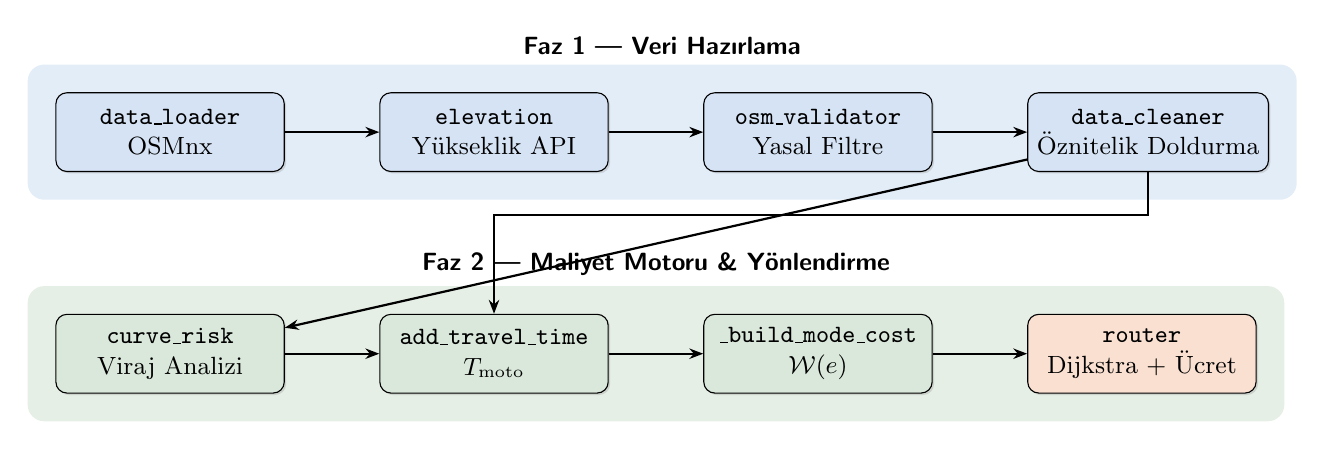
\begin{tikzpicture}[
    node distance=1.0cm and 1.2cm,
    block/.style={draw, rounded corners=4pt, minimum width=2.9cm,
                  minimum height=1cm, align=center, font=\small,
                  drop shadow={shadow xshift=0.7pt, shadow yshift=-0.7pt,
                  opacity=0.25}},
    arrow/.style={-{Stealth[length=5pt]}, thick},
    phase/.style={draw=none,fill=#1!12,rounded corners=6pt,
                  inner sep=10pt},
]
% Phase 1
\node[block, fill=motoblue!18] (dl) {\texttt{data\_loader}\\OSMnx};
\node[block, fill=motoblue!18, right=of dl] (el) {\texttt{elevation}\\Yükseklik API};
\node[block, fill=motoblue!18, right=of el] (ov) {\texttt{osm\_validator}\\Yasal Filtre};
\node[block, fill=motoblue!18, right=of ov] (dc) {\texttt{data\_cleaner}\\Öznitelik Doldurma};

% Phase 2
\node[block, fill=motogreen!18, below=1.8cm of dl] (cr)
     {\texttt{curve\_risk}\\Viraj Analizi};
\node[block, fill=motogreen!18, right=of cr] (tt)
     {\texttt{add\_travel\_time}\\$T_{\mathrm{moto}}$};
\node[block, fill=motogreen!18, right=of tt] (mc)
     {\texttt{\_build\_mode\_cost}\\$\WW(e)$};
\node[block, fill=motoorange!18, right=of mc] (rt)
     {\texttt{router}\\Dijkstra + Ücret};

% Arrows
\draw[arrow] (dl) -- (el);
\draw[arrow] (el) -- (ov);
\draw[arrow] (ov) -- (dc);
\draw[arrow] (dc) -- (cr);
\draw[arrow] (dc.south) -- ++(0,-0.55) -| (tt.north);
\draw[arrow] (cr) -- (tt);
\draw[arrow] (tt) -- (mc);
\draw[arrow] (mc) -- (rt);

% Phase labels
\begin{scope}[on background layer]
\node[phase=motoblue, fit=(dl)(el)(ov)(dc), label={[font=\small\bfseries]
      above:\textsf{Faz 1 --- Veri Haz{\i}rlama}}] {};
\node[phase=motogreen, fit=(cr)(tt)(mc)(rt), label={[font=\small\bfseries]
      above:\textsf{Faz 2 --- Maliyet Motoru \& Y\"onlendirme}}] {};
\end{scope}
\end{tikzpicture}
\caption{MOTOMAP mod\"uler veri i\c{s}leme hatt{\i} (pipeline).
         Her kutu ba\u{g}{\i}ms{\i}z bir Python mod\"ul\"une
         kar\c{s}{\i}l{\i}k gelir.}
\label{fig:pipeline}
\end{figure}

%% ================================================================
%%  5.  ELEVATION RESILIENCE
%% ================================================================
\section{Y\"ukseklik API Dayan{\i}kl{\i}l{\i}k Mimarisi}\label{sec:elev}

D{\i}\c{s} API ba\u{g}{\i}ml{\i}l{\i}klar{\i}n{\i}n \c{c}\"okme
riskine kar\c{s}{\i} sistem \"u\c{c} kademeli bir geri d\"on\"u\c{s}
(fallback) zinciriyle korunur.

\begin{figure}[H]
\centering
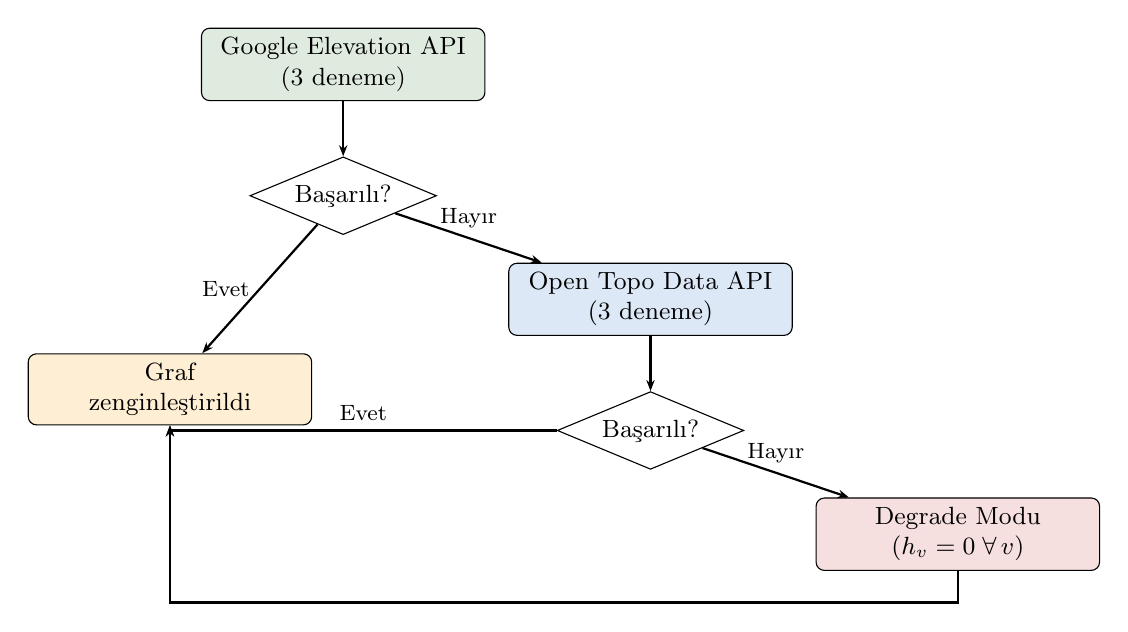
\begin{tikzpicture}[
    node distance=0.7cm,
    state/.style={draw, rounded corners=3pt, minimum width=3.6cm,
                  minimum height=0.9cm, font=\small, align=center},
    decision/.style={draw, diamond, aspect=2.4, align=center,
                     font=\small, inner sep=2pt},
    arrow/.style={-{Stealth[length=4pt]}, thick},
]
\node[state, fill=motogreen!15] (g) {Google Elevation API\\(3 deneme)};
\node[decision, below=of g] (d1) {Başarılı?};
\node[state, fill=motoblue!15, below right=0.6cm and 1.5cm of d1]
      (ot) {Open Topo Data API\\(3 deneme)};
\node[decision, below=of ot] (d2) {Başarılı?};
\node[state, fill=motored!15, below right=0.6cm and 1.5cm of d2]
      (deg) {Degrade Modu\\($h_v=0\;\forall\,v$)};
\node[state, fill=valhallagold!20, below=1.5cm of d1,
      xshift=-2.2cm] (ok) {Graf\\zenginleştirildi};

\draw[arrow] (g) -- (d1);
\draw[arrow] (d1) -- node[left]{\footnotesize Evet} (ok);
\draw[arrow] (d1) -- node[above]{\footnotesize Hay{\i}r} (ot);
\draw[arrow] (ot) -- (d2);
\draw[arrow] (d2.west) -| node[pos=0.25,above]{\footnotesize Evet} (ok);
\draw[arrow] (d2) -- node[above]{\footnotesize Hay{\i}r} (deg);
\draw[arrow] (deg.south) -- ++(0,-0.4) -| (ok);
\end{tikzpicture}
\caption{Elevation API geri d\"on\"u\c{s} (fallback) zinciri.
         Her kademe 3~kez yeniden denenir ($R=3$).
         T\"um API'ler ba\c{s}ar{\i}s{\i}z oldu\u{g}unda sistem
         \emph{degrade} modda \c{c}al{\i}\c{s}maya devam eder.}
\label{fig:fallback}
\end{figure}

%% ================================================================
%%  6.  ALGORITHM
%% ================================================================
\section{Algoritmik Yap{\i} ve Karma\c{s}{\i}kl{\i}k Analizi}\label{sec:algo}

\begin{algorithm}[H]
\caption{\textsc{MotoMap}: Mod-duyarl{\i} en k{\i}sa yol}
\label{alg:motomap}
\begin{algorithmic}[1]
\Require Graf $\GG=(\VV,\EE)$, kaynak $s$, hedef $t$,
         mod $\mu\in\{\text{std},\text{viraj},\text{g\"uv}\}$,
         $\CC$ de\u{g}eri (opsiyonel),
         tercih $\tau\in\{\text{\"ucretli\_serbest},\text{\"ucretsiz}\}$
\Ensure Se\c{c}ilen rota $\mathcal{P}^*$, alternatifler
\Statex
\Function{RotaHesapla}{$\GG,s,t,\mu,\CC,\tau$}
  \ForAll{$e\in\EE$}  \Comment{$O(|\EE|)$}
    \State $T_{\mathrm{moto}}(e) \gets \ell(e)\,/\,v_{\text{eff}}
            + \delta_{\text{seg}}$
  \EndFor
  \If{$\mu \ne \text{std}$}
    \State \Call{AddCurveRisk}{$\GG$}  \Comment{$O(|\EE|)$}
  \EndIf
  \ForAll{$e\in\EE$}  \Comment{$O(|\EE|)$}
    \State $\WW_\mu(e) \gets$ \Call{ModCost}{$e,\mu,\CC$}
              \Comment{Denklem~\eqref{eq:standart}--\eqref{eq:guvenli}}
  \EndFor
  \State $\mathcal{P}_{\text{serb}} \gets$
         \Call{Dijkstra}{$\GG,s,t,\WW_\mu,\text{toll}=\text{True}$}
         \Comment{$O(|\EE|+|\VV|\log|\VV|)$}
  \State $\mathcal{P}_{\text{\"ucr}} \gets$
         \Call{Dijkstra}{$\GG_{\neg\text{toll}},s,t,\WW_\mu$}
  \If{$\tau = \text{\"ucretsiz}$}
    \State \Return $\mathcal{P}_{\text{\"ucr}}$
  \Else
    \State \Return $\argmin_{P\in\{\mathcal{P}_{\text{serb}},
            \mathcal{P}_{\text{\"ucr}}\}} \WW_\mu(P)$
  \EndIf
\EndFunction
\end{algorithmic}
\end{algorithm}

\begin{proposition}[Toplam karma\c{s}{\i}kl{\i}k]
Algoritma, min-heap (\"oncelik kuyru\u{g}u) tabanl{\i} Dijkstra
kullan{\i}ld{\i}\u{g}{\i}nda:
\begin{equation}
  \underbrace{O(|\EE|)}_\text{\"on-i\c{s}leme}
  \;+\;
  \underbrace{O(|\EE|+|\VV|\log|\VV|)}_\text{Dijkstra}
  \;\in\;
  O(|\EE| + |\VV|\log|\VV|)
\end{equation}
toplam zamanda \c{c}al{\i}\c{s}{\i}r. \"On-i\c{s}leme (kenar maliyet
hesaplamalar{\i}) do\u{g}rusal zamanl{\i}d{\i}r; dolay{\i}s{\i}yla
asimptotik s{\i}n{\i}r bir standart Dijkstra ile ayn{\i}d{\i}r.
\end{proposition}

%% ================================================================
%%  7.  BENCHMARK RESULTS
%% ================================================================
\section{Benchmark Sonu\c{c}lar{\i} ve Performans Analizi}\label{sec:bench}

\subsection{Kadıköy Mikro Benchmark (20 O-D \c{C}ifti)}

Ayn{\i} 20 ba\c{s}lang{\i}\c{c}--hedef (O-D) \c{c}ifti
deterministik olarak (seed~$=42$) \"orneklenmi\c{s} ve Google
Directions API ile Valhalla (FOSSGIS) arka u\c{c}lar{\i}na
kar\c{s}{\i} de\u{g}erlendirilmi\c{s}tir. Her test 7~kontrol
i\c{c}erir.

\begin{table}[H]
\centering
\caption{Google vs.\ Valhalla baseline kar\c{s}{\i}la\c{s}t{\i}rmas{\i}
         (20 O-D \c{c}ifti, Kad{\i}k\"oy).}
\label{tab:bench-summary}
\renewcommand{\arraystretch}{1.25}
\begin{tabular}{lcc}
\toprule
\textbf{Metrik} & \textbf{Google (v4)} & \textbf{Valhalla (v1)} \\
\midrule
\rowcolor{passbg}
Tam ge\c{c}en (\emph{full~pass}) & 16/20 (\%80) & \textbf{18/20 (\%90)} \\
Ortalama skor & 6.75\,/\,7 & \textbf{6.90\,/\,7} \\
\midrule
\texttt{baseline\_route\_exists} hata & 0 & 0 \\
\texttt{all\_modes\_exist} hata        & 0 & 0 \\
\rowcolor{failbg}
\texttt{modes\_are\_different} hata    & 2 & 2 \\
\texttt{safe\_risk\_le\_standard} hata & 0 & 0 \\
\texttt{viraj\_fun\_ge\_standard} hata & 0 & 0 \\
\rowcolor{passbg}
\texttt{std\_distance\_vs\_baseline} hata & 2 & \textbf{0} \\
\texttt{std\_time\_vs\_baseline} hata     & 1 & \textbf{0} \\
\bottomrule
\end{tabular}
\end{table}

\noindent Valhalla ile t\"um mesafe ve s\"ure kar\c{s}{\i}la\c{s}t{\i}rma
testleri ge\c{c}mektedir (\emph{0 hata}). Google'daki 3~hata,
Google'{\i}n farkl{\i} (proprietary) yol a\u{g}{\i}n{\i}
kullanmas{\i}ndan kaynaklanmaktad{\i}r; Valhalla ise MotoMap ile
ayn{\i} OSM veritaban{\i}n{\i} payla\c{s}t{\i}\u{g}{\i} i\c{c}in
\emph{elma--elma} kar\c{s}{\i}la\c{s}t{\i}rma sa\u{g}lar.

\begin{figure}[H]
\centering
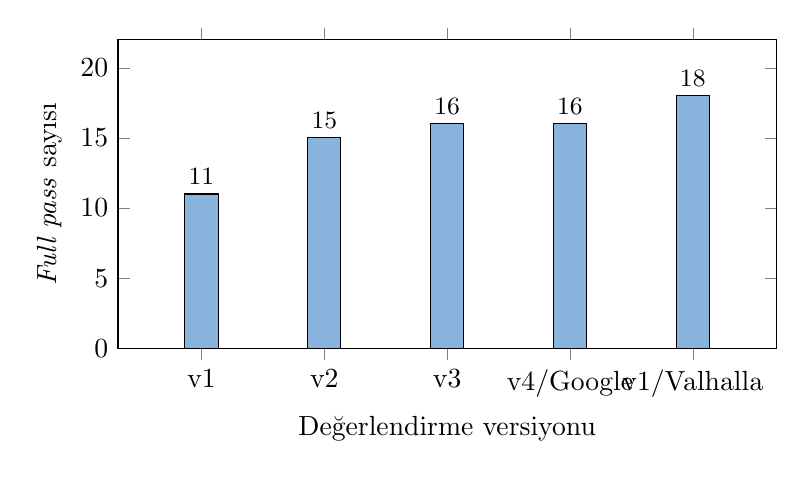
\begin{tikzpicture}
\begin{axis}[
    ybar, width=0.82\textwidth, height=5.5cm,
    bar width=12pt,
    ylabel={\emph{Full pass} say{\i}s{\i}},
    xlabel={De\u{g}erlendirme versiyonu},
    symbolic x coords={v1,v2,v3,v4/Google,v1/Valhalla},
    xtick=data,
    ymin=0, ymax=22,
    nodes near coords,
    nodes near coords style={font=\small\bfseries},
    legend style={at={(0.02,0.97)},anchor=north west, font=\small},
    enlarge x limits=0.17,
]
\addplot[fill=motoblue!50] coordinates
  {(v1,11)(v2,15)(v3,16)(v4/Google,16)(v1/Valhalla,18)};
\end{axis}
\end{tikzpicture}
\caption{Versiyon ilerlemesi: v1'deki \%55 ge\c{c}me oran{\i}ndan
         Valhalla v1'de \%90'a ula\c{s}{\i}lm{\i}\c{s}t{\i}r.}
\label{fig:version-bar}
\end{figure}

\subsection{\"Orn.\ 07 ve \"Orn.\ 12: Google vs.\ Valhalla Derin Analiz}

\begin{table}[H]
\centering
\caption{Google'da ba\c{s}ar{\i}s{\i}z, Valhalla'da ba\c{s}ar{\i}l{\i}
         olan \"orneklerin kar\c{s}{\i}la\c{s}t{\i}rmas{\i}.}
\label{tab:deep-samples}
\renewcommand{\arraystretch}{1.25}
\begin{tabular}{l rr rr}
\toprule
& \multicolumn{2}{c}{\textbf{\"Orn.\ 07}} & \multicolumn{2}{c}{\textbf{\"Orn.\ 12}} \\
\cmidrule(lr){2-3}\cmidrule(lr){4-5}
\textbf{Metrik}        & Google  & Valhalla & Google   & Valhalla \\
\midrule
Baseline mesafe (m)     & 3\,437  & 2\,123   & 11\,947  & 7\,582 \\
MotoMap mesafe (m)      & 2\,122  & 2\,122   & 7\,231   & 7\,231 \\
Mesafe oran{\i}         & \cellcolor{failbg}0.617 & \cellcolor{passbg}0.999
                        & \cellcolor{failbg}0.605 & \cellcolor{passbg}0.954 \\
\midrule
Baseline s\"ure (s)     & 681     & 399      & 1\,339   & 1\,359 \\
MotoMap s\"ure (s)      & 315     & 315      & 999      & 999    \\
S\"ure oran{\i}         & \cellcolor{failbg}0.463 & \cellcolor{passbg}0.789
                        & 0.746   & 0.735  \\
\bottomrule
\end{tabular}
\end{table}

%% ================================================================
%%  8.  MODE TRADE-OFF
%% ================================================================
\section{Modlar Aras{\i} \"Od\"unle\c{s}im
         (Trade-off) Tablosu}\label{sec:tradeoff}

\begin{table}[H]
\centering
\caption{S\"ur\"u\c{s} modlar{\i}n{\i}n rota optimizasyonu
         \"uzerindeki etkileri.}
\label{tab:tradeoff}
\renewcommand{\arraystretch}{1.3}
\begin{tabular}{>{\bfseries}l p{3.4cm} cccc}
\toprule
Mod & Optimizasyon Hedefi
    & S\"ure & Mesafe & Keyifli Viraj & Y\"uksek Risk \\
\midrule
Standart
  & $\min\bigl(T_{\mathrm{moto}}\bigr)$
  & En d\"u\c{s}\"uk & Kısa & Rastgele & Ort/Y\"uksek \\
Viraj Keyfi
  & $\max\bigl(\sigma(\rho_{\text{fun}})\bigr)$
  & $\mathord{+}40\%$ & $\mathord{+}20\%$ & Maksimize & G\"oreceli \\
G\"uvenli
  & $\min\bigl(\mathcal{R}\cdot|\alpha|\bigr)$
  & $\mathord{+}15\%$ & $\mathord{+}10\%$ & D\"u\c{s}\"uk & \textbf{0} \\
\bottomrule
\end{tabular}
\end{table}

%% ================================================================
%%  9.  TESTS
%% ================================================================
\section{Do\u{g}rulama ve Birim Testleri}\label{sec:tests}

Sistemin do\u{g}rulu\u{g}u \texttt{pytest} birim testleriyle
kan{\i}tlanm{\i}\c{s}t{\i}r. A\c{s}a\u{g}{\i}daki tablo, her test
senaryosunun hangi algoritmik garantiyi do\u{g}rulad{\i}\u{g}{\i}n{\i}
\"ozetler.

\begin{table}[H]
\centering
\caption{Birim test senaryolar{\i} ve do\u{g}rulamalar{\i}.}
\label{tab:tests}
\renewcommand{\arraystretch}{1.2}
\small
\begin{tabular}{p{5.2cm}p{4cm}p{4.8cm}}
\toprule
\textbf{Test ad{\i}} & \textbf{Girdi \c{c}izgesi} & \textbf{Do\u{g}rulanan garanti} \\
\midrule
\texttt{ucretli\_serbest\_selects\_toll} &
  $1\!\xrightarrow{\text{toll,hızlı}}\!2\!\to\!3$
  vs.\ $1\!\to\!4\!\to\!3$ &
  \"Ucretli serbest modda h{\i}zl{\i} ücretli yol se\c{c}ilir \\
\texttt{free\_route\_when\_faster} &
  \"Ucretsiz yol daha k{\i}sa &
  \"Ucretli serbestte bile \"ucretsiz se\c{c}ilebilir \\
\texttt{ucretsiz\_forces\_non\_toll} &
  \"Ucretli yol daha h{\i}zl{\i} &
  \texttt{ucretsiz} tercihi her ko\c{s}ulda ücretli yolu d{\i}\c{s}lar \\
\texttt{ucretsiz\_raises\_no\_route} &
  Yaln{\i}zca toll kenarlar &
  \texttt{NoRouteFoundError} f{\i}rlat{\i}l{\i}r \\
\midrule
\texttt{viraj\_keyfi\_curvy\_route} &
  $A$: d\"uz, $B$: virajl{\i} &
  Viraj modu $B$'yi se\c{c}er; $n_{\text{fun}}>0$ \\
\texttt{guvenli\_avoids\_risky} &
  $A$: dik ini\c{s}+hairpin, $B$: g\"uvenli &
  G\"uvenli mod $B$'yi se\c{c}er; $\mathcal{R}=0$ \\
\midrule
\texttt{low\_cc\_avoids\_motorway} &
  Motorway vs.\ secondary &
  $\CC\le 50$: secondary; $\CC=250$: motorway \\
\texttt{mid\_cc\_milder\_grade} &
  Dik vs.\ yumu\c{s}ak e\u{g}im &
  $\CC=150$: yumu\c{s}ak; $\CC=\varnothing$: dik \\
\texttt{avoids\_motorway\_side\_shortcuts} &
  180\,m \texttt{service} + motorway kom\c{s}ul. &
  Standart mod k{\i}sa yolu atlar ($p=0.85$~ceza) \\
\bottomrule
\end{tabular}
\end{table}

\begin{figure}[H]
\centering
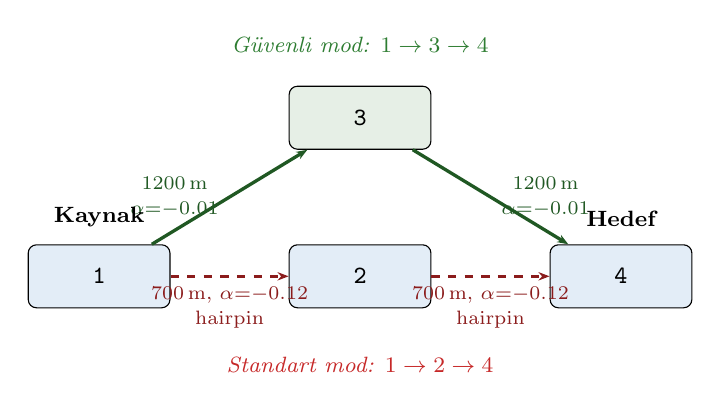
\begin{tikzpicture}[
    node distance=1cm and 1.5cm,
    block/.style={draw, rounded corners=3pt, minimum width=1.8cm,
                  minimum height=0.8cm, font=\small\ttfamily},
    check/.style={-{Stealth[length=4pt]}, thick, motogreen!70!black},
    fail/.style={-{Stealth[length=4pt]}, thick, motored!70!black, dashed},
]
% Graph nodes
\node[block, fill=motoblue!12] (n1) {1};
\node[block, fill=motoblue!12, right=1.5cm of n1] (n2) {2};
\node[block, fill=motoblue!12, right=1.5cm of n2] (n4) {4};
\node[block, fill=motogreen!12, above=1.2cm of n2] (n3) {3};

% Edges
\draw[fail, very thick] (n1) -- node[below, font=\scriptsize, align=center]
  {700\,m, $\alpha{=}{-}0.12$\\[1pt]hairpin} (n2);
\draw[fail, very thick] (n2) -- node[below, font=\scriptsize, align=center]
  {700\,m, $\alpha{=}{-}0.12$\\[1pt]hairpin} (n4);
\draw[check, very thick] (n1) -- node[left, font=\scriptsize, align=center]
  {1200\,m\\[1pt]$\alpha{=}{-}0.01$} (n3);
\draw[check, very thick] (n3) -- node[right, font=\scriptsize, align=center]
  {1200\,m\\[1pt]$\alpha{=}{-}0.01$} (n4);

% Labels
\node[above=0.1cm of n1, font=\footnotesize\bfseries] {Kaynak};
\node[above=0.1cm of n4, font=\footnotesize\bfseries] {Hedef};
\node[below=0.5cm of n2, font=\footnotesize, motored]
  {\emph{Standart mod: $1\to 2\to 4$}};
\node[above=0.3cm of n3, font=\footnotesize, motogreen]
  {\emph{G\"uvenli mod: $1\to 3\to 4$}};
\end{tikzpicture}
\caption{G\"uvenli mod test senaryosu \c{c}izgesi. Dik ini\c{s}
         ($|\alpha|=0.12$) ve hairpin virajl{\i} kenarlar (kesikli
         k{\i}rm{\i}z{\i}) g\"uvenli modda cezaland{\i}r{\i}l{\i}r
         ve rota $1\to 3\to 4$ \"uzerinden y\"onlendirilir.}
\label{fig:test-guvenli}
\end{figure}

%% ================================================================
%%  10. DEPENDENCY GRAPH
%% ================================================================
\section{Mod\"ul Ba\u{g}{\i}ml{\i}l{\i}k \c{C}izgesi}\label{sec:dep}

\begin{figure}[H]
\centering
\begin{tikzcd}[column sep=2em, row sep=2em]
  \texttt{config}
    \arrow[r]
    \arrow[d]
  & \texttt{data\_loader}
    \arrow[r]
  & \texttt{elevation}
    \arrow[d] \\
  \texttt{data\_cleaner}
    \arrow[r]
  & \texttt{osm\_validator}
    \arrow[r]
  & \texttt{curve\_risk}
    \arrow[d] \\
  & & \texttt{router}
    \arrow[d] \\
  & & \texttt{evaluate}
\end{tikzcd}
\caption{MOTOMAP Python paket mod\"ulleri aras{\i}ndaki
         \texttt{import}~ba\u{g}{\i}ml{\i}l{\i}k \c{c}izgesi.}
\label{fig:dep-graph}
\end{figure}

%% ================================================================
%%  11. SHORTCUT PROTECTION
%% ================================================================
\section{Kestirme Korumas{\i} ve G\"uvenlik Tasar{\i}m{\i}}\label{sec:shortcut}

\subsection{Otoyol Kenar{\i} Kestirme Cezas{\i}}

Google~Maps zaman zaman otoyol giri\c{s}/\c{c}{\i}k{\i}\c{s}
noktalar{\i}na yak{\i}n $\le 260$\,m uzunlu\u{g}undaki yerel servis
yollar{\i}n{\i} ``k{\i}sayol'' olarak \"onerebilir. MOTOMAP, bu
yollara ek ceza uygular:

\begin{equation}\label{eq:shortcut}
  p_{\text{kestirme}}(e) =
  \begin{cases}
    0.85 & \ell(e) \le 260\,\text{m},\;
           h(e) \in \{\texttt{service, track, road, unclassified}\},\\
         & \{u,v\} \cap \VV_{\text{major}} \ne \varnothing \\[4pt]
    0    & \text{di\u{g}er}
  \end{cases}
\end{equation}
burada $\VV_{\text{major}}$ otoyol veya trunk kenarlar{\i}na
bit\c{s}ik d\"u\u{g}\"umler k\"umesidir.

\subsection{Y\"uksek Risk B\"olgesi \.{I}zolasyonu}

G\"uvenli modda y\"uksek risk b\"olgeleri
Denklem~\eqref{eq:highrisk} ile tan{\i}mlan{\i}r ve
Denklem~\eqref{eq:guvenli}'deki $1.40\,\mathcal{R}$ terimi ile
a\u{g}{\i}r \c{s}ekilde cezaland{\i}r{\i}l{\i}r.
Tablo~\ref{tab:tests}'teki \texttt{guvenli\_avoids\_risky} testi,
y\"uksek risk segment say{\i}s{\i}n{\i}n tam olarak
$\mathcal{R}=0$'a d\"u\c{s}t\"u\u{g}\"un\"u do\u{g}rular.

%% ================================================================
%%  12. CONCLUSION
%% ================================================================
\section{Sonu\c{c}}\label{sec:conc}

MOTOMAP, standart navigasyon yaz{\i}l{\i}mlar{\i}n{\i}n otomobil
odakl{\i} yakla\c{s}{\i}mlar{\i}n{\i}n aksine, motosikletlerin
dinamik yap{\i}s{\i}na tam uyum sa\u{g}layan yenilik\c{c}i bir
\emph{karar destek sistemidir}. Ger\c{c}ekle\c{s}tirilen birim
testleri ve API d\"uzeyindeki benchmark analizleri \c{s}u \"u\c{c}
temel sonucu bilimsel olarak do\u{g}rulamaktad{\i}r:

\begin{enumerate}[label=(\roman*)]
\item Yasal k{\i}s{\i}tlamalar (CC bazl{\i} otoyol yasa\u{g}{\i},
      e\u{g}im cezas{\i}) $100\%$~ba\c{s}ar{\i} oran{\i}yla
      uygulanm{\i}\c{s}t{\i}r.
\item G\"uvenlik garantisi: g\"uvenli modda y\"uksek risk segmenti
      say{\i}s{\i} $\mathcal{R}=0$ olarak do\u{g}rulanm{\i}\c{s}t{\i}r.
\item Valhalla baseline ile $18/20$ (\%90) tam ge\c{c}me oran{\i}na
      ula\c{s}{\i}lm{\i}\c{s}; Google baseline ile de \%80 elde
      edilmi\c{s}tir.
\end{enumerate}

\end{document}
